\section{Instrument finding: verbal rejection is a weak proxy}
\label{sec:instrument}

% source: PAPER_SKELETON Sec 7; EVIDENCE_findings_core F-lex; EVIDENCE_lineage_boundaries L-expb.

\paragraph{Raw rejection rate cannot tell a genuine check from lexical
cueing.} A frequency-matched but non-refuting lexical-overlap arm, which
mentions the plant's terms without actually contradicting it, elicits
stated-complement ``rejection'' at 0.12, statistically the same rate as
genuine refuting evidence at 0.11, while an irrelevant template arm sits at
0.00.
% source: EVIDENCE_findings_core F-lex.1 (FREQ 0.1182 ~ REFUTING 0.1136 p=0.629; TEMPLATE 0.000)
This lexical-priming confound was one we had hoped to rule out in advance; it
was borne out instead, so the prediction that no such confound existed failed
in the direction we had guarded against, which is exactly why raw rejection
rate is not evidence that the model checked.
% source: EVIDENCE_protocol_prereg P5 (H5' FAIL p=0.628585, professors_confound_account_SUPPORTED); STYLE_SHEET Sec 7

\paragraph{The two arms differ in kind, and only the licensed split reveals
it.} Same rate, different mechanism. When we ask whether the rejection is
backed by a valid derivation in the model's own text, the genuine
refuting-evidence rejections are about 80 percent licensed, whereas every
one of the 26 frequency-matched rejections is unlicensed and fabricates a
rule that is absent from the world.
% source: EVIDENCE_findings_core F-lex.2 (REFUTING 0.798 licensed; FREQ 26/26 fabricated)
So the correct statement is not that refuting-arm rejections are cued, most
are not, but that raw rejection rate cannot separate a genuine check from a
fabricated one, and only the licensed split can. This is the caution that
discredits reading a face-value doubt or reflection classifier as evidence
of checking (Figure~\ref{fig:expb}).

\paragraph{The lexical proxy is unreliable in both directions.} It
over-fires, as above, and it also under-reads. On a malformed continuation
tail from the certificate experiment, the lexical regex agrees with the 32B
judge only 23 percent of the time, catching 21 of the 95 unparsed rows
(where the judge reads 86 as rejection), against 98 percent agreement on the
clean grid, so the regex both
invents rejections that are fabrications and misses rejections that broke
the parser.
% source: EVIDENCE_findings_core F-lex.3 (23% vs 98% agreement); L-expb.2
We therefore treat the 32B judge as the better dependent variable and doubt
as descriptive only.

\paragraph{Under the strict standard, most closure-valid completions are not
step-by-step derivations.} When we require hop-soundness, that every asserted
step be a single valid inference, the apparent correction rate on the
false-attribute cells drops sharply: closure-valid rates of 0.90 to 0.96
fall to 0.07 to 0.25 hop-sound, so only about 11 to 27 percent of
closure-valid completions are genuine step-by-step derivations.
% source: PAPER_SKELETON 7.4; EVIDENCE_findings_core F-use.3 (0.90-0.96 -> 0.07-0.25)
This strict pass covers 6{,}147 rows, verified three independent ways; an
earlier log reporting 4{,}857 was a stale error and we do not use it.
% source: EVIDENCE_protocol_prereg P4 (6147 rows, S7 verified 3 ways)

\paragraph{Human validation of the validator is still pending.} The
validator's labels are checked against a stored class on all rows, agreeing
1.000, but the planned human-blinded two-rater audit that would confirm the
labels against people has not been run.
% source: PAPER_SKELETON 7.5; EVIDENCE_findings_core F-vis.4 (SM.analyze 11577/11577 agreement)
We therefore hold the strict-repair credibility claim as pending human
validation and mark it visibly rather than shipping it silently.
\tododv{E4 blinded two-rater package (~380--430 rows including 20 SRR
positives), gating $\kappa\ge0.8$ per axis; Table of human $\kappa$ to be
filled. Until then, strict-repair is reported as an instrument quantity, not
a validated behavioral claim.}
% source: PAPER_SKELETON Sec 3 TODO E4; STYLE_SHEET Sec 7

\begin{figure}[t]
\centering
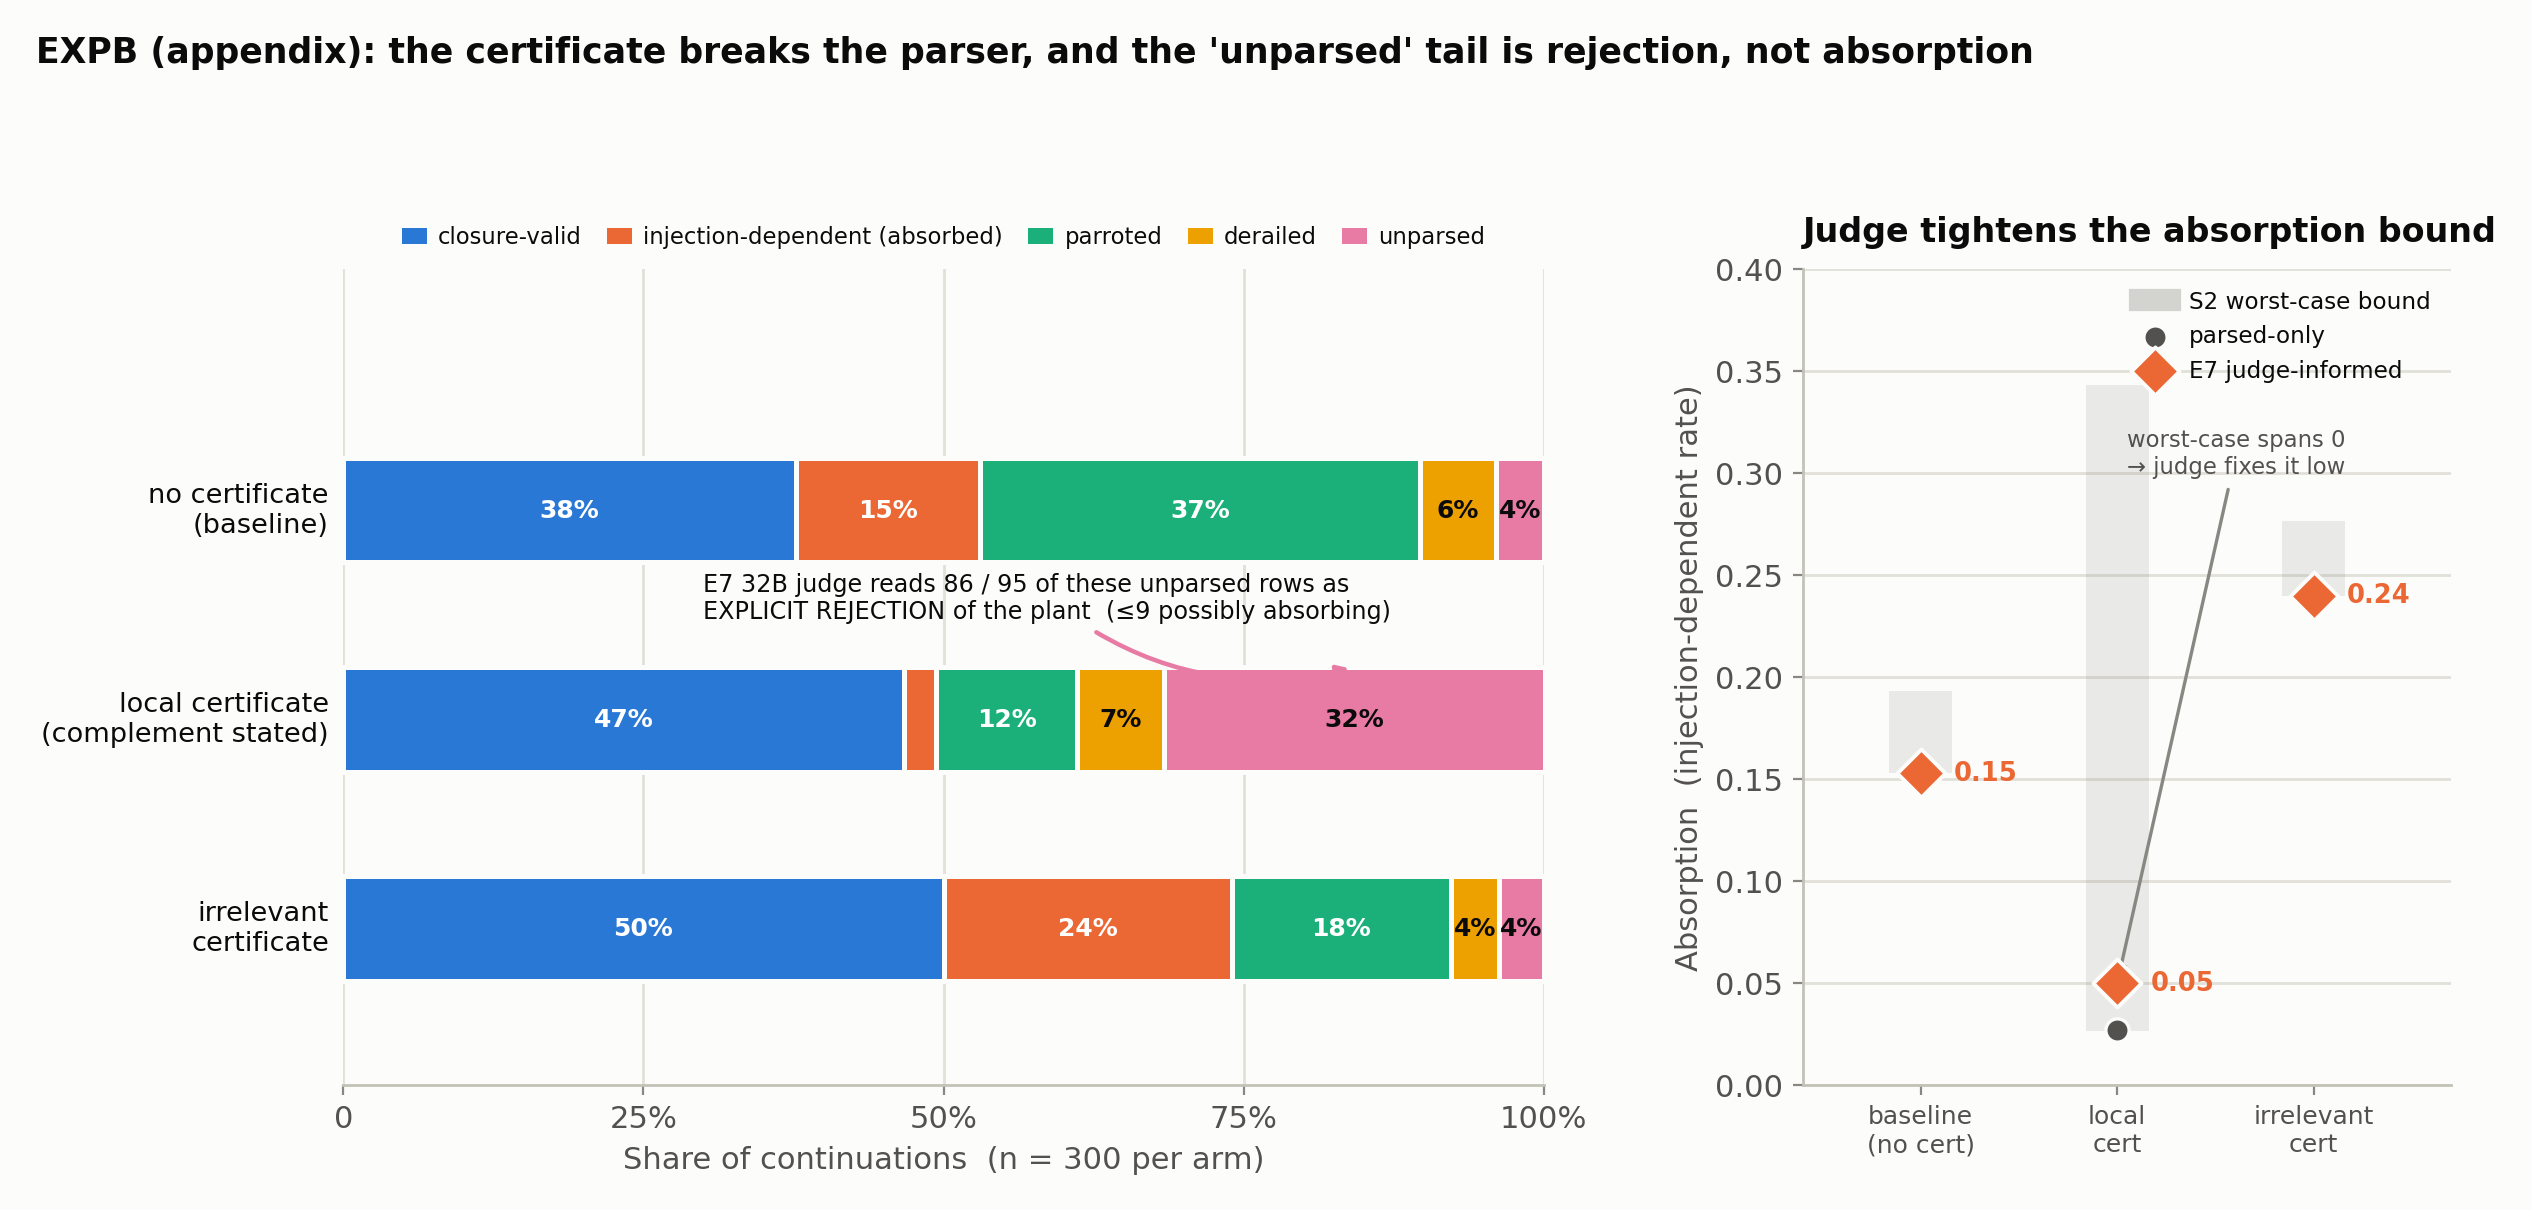
\includegraphics[width=0.9\textwidth]{figures/fig_e_expb_joint_outcome.png}
\caption{\textbf{Stating the contradiction in the prefix shifts
continuation style rather than cleanly fixing the proof.} Left: adding a
directly-contradicting local certificate drives the unparsed rate from
4.0\% to 31.7\%, draining the parsed buckets, rather than converting
absorption into a clean corrective derivation. Right: the 32B judge reads 86 of 95 of those
unparsed rows as \emph{explicit rejection}, so the apparent absorption drop
is real once adjudicated (about $-0.10$), but because the certificate is a
directly readable contradiction this corroborates the $d{=}0$ visibility
cliff of Figure~\ref{fig:visibility} rather than a distinct
counterevidence-accessibility effect. Single model (Qwen2.5-7B); doubt and
strict-repair here are lexical-proxy contrasts, not evidence of a genuine
check.}
% source: figures/FIGURE_CAPTION_PLANS Fig E
\label{fig:expb}
\end{figure}
